\section{The analytic construction}\label{sec:analytic-construction}

We prove Proposition~\ref{prop:analytic-model} by compactifying the torus
family determined by $\Lambda^+$ over the three marked points of $B$.
The rational monodromy operators and the holomorphic period functions from
\citep[Sections~2--3]{Alpoge2026} are retained; what changes is the integral
marking.  The proof is therefore organized around the three places where
that marking enters the construction.  We first check that the finite
monodromies preserve $\Lambda^+$ and admit free affine lifts.  We then
rewrite the period matrix in the new marking.  Finally, we compactify its
logarithmic term at the cusp, where the deck-translation lattice has index
two in the toric lattice.  Once these compatibility statements are in
place, it remains to identify the local models over the punctured coordinate
discs and glue them.  The period-function lemma used below is proved in
Appendix~\ref{app:period-torsor}.

\subsection{The enlarged lattice and the finite monodromies}

Let $B=\PP^1$, with $p_1=0$, $p_2=1$, and $p_0=\infty$, and let
$t$ be the affine coordinate on $B\setminus\{p_0\}$.  Following
\citep[Section~2.1]{Alpoge2026}, let
$\Lambda=\ZZ\langle\widehat\gamma,\widehat u,\widehat w,
\widehat\delta\rangle$ and
$\mathcal B=(\widehat\gamma,\widehat u,\widehat w,\widehat\delta)$.
Let $A_1,A_2\in\operatorname{Aut}(\Lambda)$ be the monodromy operators
about $p_1,p_2$.  With the column-vector convention, their matrices in
the ordered basis $\mathcal B$ are
\begin{equation}\label{eq:an-original-monodromy-matrices}
 [A_1]_{\mathcal B}=
 \begin{pmatrix}
 1&0&0&0\\
 6&0&1&0\\
 -6&-1&-1&0\\
 -2&1&0&1
 \end{pmatrix},
 \qquad
 [A_2]_{\mathcal B}=
 \begin{pmatrix}
 1&0&0&0\\
 0&0&-1&0\\
 -6&1&0&0\\
 3&0&1&1
 \end{pmatrix}.
\end{equation}
These monodromy operators and the translation vectors used below are taken
from \citep[Lemmas~2.4 and~2.6]{Alpoge2026}.  Our task is to find an
overlattice that they preserve and that has the required cusp behaviour.

To make that requirement precise, let $K$ denote the cocharacter lattice
of the torus used in the cusp compactification and let $L\subset K$ be the
lattice of deck translations.  The irreducible components of the central
fibre are indexed by $K/L$.  For $\Lambda$, the lattice $L$ is
saturated in $K$, and the central fibre has one component.  To obtain the
divisor data needed for nonzero second cohomology, we require two components,
hence $[K:L]=2$.  We therefore seek the smallest monodromy-invariant
enlargement of $\Lambda$ for which the logarithmic period matrix has this
index.  Every index-two overlattice of
$\Lambda$ lies in $\tfrac12\Lambda$ and has the form
$\Lambda+\mathbb Z(v/2)$ for a nonzero class
$\bar v\in\Lambda/2\Lambda$.  Reducing
\eqref{eq:an-original-monodromy-matrices} modulo two gives
\[
 \begin{aligned}
 \ker(\bar A_1-I)
  &=\mathbb F_2\langle\overline{\widehat\gamma},
       \overline{\widehat\delta}\rangle,\\
 \ker(\bar A_2-I)
  &=\mathbb F_2\langle
       \overline{\widehat\gamma+\widehat u+\widehat w},
       \overline{\widehat\delta}\rangle,
 \end{aligned}
 \qquad
 \ker(\bar A_1-I)\cap\ker(\bar A_2-I)
 =\mathbb F_2\,\overline{\widehat\delta}
 \subset\Lambda/2\Lambda.
\]
Thus the only possible new half-period is represented by
$\widehat\delta/2$.  Put
$d=\widehat\delta/2\in\Lambda\otimes\mathbb Q$ and
$\Lambda^+=\Lambda+\ZZ d
=\ZZ\langle\widehat\gamma,\widehat u,\widehat w,d\rangle$.
Then $[\Lambda^+:\Lambda]=2$, and $\Lambda^+$ is the unique index-two
overlattice of $\Lambda$ preserved by both monodromy operators.

Write $\mathcal B^+=(\widehat\gamma,\widehat u,\widehat w,d)$ and
$D=\operatorname{diag}(1,1,1,\tfrac12)$.
The columns of $D$ are the vectors of $\mathcal B^+$, expressed in
the basis $\mathcal B$.  The change-of-basis formula therefore gives
\begin{equation}\label{eq:an-monodromy-matrices}
 \begin{aligned}
 [A_1]_{\mathcal B^+}
 &
 =\begin{pmatrix}
  1&0&0&0\\
  6&0&1&0\\
  -6&-1&-1&0\\
  -4&2&0&1
 \end{pmatrix},
 [A_2]_{\mathcal B^+}
 &
 =\begin{pmatrix}
  1&0&0&0\\
  0&0&-1&0\\
  -6&1&0&0\\
  6&0&2&1
 \end{pmatrix}.
 \end{aligned}
\end{equation}
In particular, these matrices are integral, which verifies directly that
$A_1$ and $A_2$ preserve $\Lambda^+$.  The operators on
$\Lambda\otimes\mathbb Q=\Lambda^+\otimes\mathbb Q$ have not changed;
only their coordinate matrices have changed.  All subsequent coordinate
formulas for the monodromy use the basis $\mathcal B^+$.
The affine translation vectors are
$v_1=\widehat\gamma+2\widehat u-4\widehat w$ and
$v_2=-\widehat\gamma-3\widehat u+3\widehat w$.
Let $m_1=3$, $m_2=4$, and let
$\gamma\in\operatorname{Hom}(\Lambda^+,\ZZ)$ be dual to
$\widehat\gamma$.  The local model over $p_j$ will be obtained from the
affine transformation $x\longmapsto A_jx+v_j/m_j$ on
$(\Lambda^+\otimes\mathbb R)/\Lambda^+$.
These data give a cyclic action of order $m_j$ provided
$A_j^{m_j}=I$ and $A_jv_j=v_j$; its $m_j$-th power is then translation
by the period $v_j$.  Freeness can be checked by finding an
$A_j$-invariant integral character $\gamma$ for which
$\gcd(\gamma(v_j),m_j)=1$.  Direct multiplication gives
\begin{equation}\label{eq:an-finite-orders}
 A_1^3=A_2^4=I,
 \qquad A_jv_j=v_j,
 \qquad \gamma\circ A_j=\gamma\quad (j=1,2),
 \qquad \gamma(v_1)=1,\quad\gamma(v_2)=-1.
\end{equation}% display-paragraph-boundary: intentional new paragraph follows

Indeed, if the $k$-th power, with $0<k<m_j$, had a fixed point, applying
$\gamma$ to the fixed-point equation would give
$k\gamma(v_j)/m_j\in\mathbb Z$, a contradiction.  Thus
\eqref{eq:an-finite-orders} records exactly the properties of the existing
monodromy data needed after the change of lattice.  We use this criterion
explicitly in the construction of the two multiple fibres.

\subsection{Period functions and equivariance}

The matrices $[A_j]_{\mathcal B^+}$ in
\eqref{eq:an-monodromy-matrices} prescribe the integral monodromy.  To
realize them by a holomorphic family of complex tori, we need a period matrix
$\Pi^+$ and
holomorphic changes of fibre coordinates $R_j(z)\in\operatorname{GL}_2(\CC)$
satisfying $R_j(z)\Pi^+(z)=\Pi^+(g_jz)A_j$.
The functions in the next lemma provide such a matrix.  Their cusp
normalization also separates its logarithmic term from the part that extends
holomorphically across $p_0$.

Let $\Gamma_{\mathrm{orb}}
=\langle g_1,g_2\mid g_1^3=g_2^4=1\rangle$, with
$g_0=(g_1g_2)^{-1}$, act on $\mathfrak H_z$, and let
$\pi:\mathfrak H_z\to B\setminus\{p_0\}$ be the resulting orbifold
uniformization.  If $z_j$ is fixed by
$g_j$, choose the generator orientations and linearizing coordinates so
that $s_j(g_jz)=e^{-2\pi i/m_j}s_j(z)$, where
$(m_1,m_2)=(3,4)$.
Let $U_0^\times$ be a punctured disc about $p_0$, and choose a connected
component $\widetilde U_0$ of $\pi^{-1}(U_0^\times)$ whose stabilizer is
$\langle g_0\rangle$.

\begin{lemma}[Period functions]\label{lem:an-period-functions}
There are holomorphic functions
$\tau:\mathfrak H_z\to\mathfrak H$ and
$\mu,\beta:\mathfrak H_z\to\CC$ satisfying
\begin{align}
 \tau(g_1z)&=\frac{\tau-1}{\tau},
 &\tau(g_2z)&=-\frac1\tau,\label{eq:an-tau-laws}\\
 \mu(g_1z)&=\frac{1-\mu}{\tau},
 &\mu(g_2z)&=1+(\mu/\tau),\label{eq:an-mu-laws}\\
 \beta(g_1z)&=\beta+2-\frac{6(1-\mu)^2}{\tau},
 &\beta(g_2z)&=\beta-3-\frac{6\mu^2}{\tau}.
 \label{eq:an-beta-laws}
\end{align}
Here and below, functions without a displayed argument are evaluated at
$z$.  These laws imply $\tau(g_0z)=\tau-1$,
$\mu(g_0z)=\mu$, and $\beta(g_0z)=\beta+1$.
If $t_c=t^{-1}$, then on $\widetilde U_0$ there are a
logarithmic coordinate $s$ and a function $h$, holomorphic in $t_c$
at zero, such that
\begin{equation}\label{eq:an-log-coordinate}
 e^{2\pi is}=t_c,
 \qquad s(g_0z)=s(z)-1,
 \qquad \tau=s+h(t_c),
\end{equation}
and $\mu$ and $b_c:=\beta+\tau$ are holomorphic in $t_c$ at zero.
The additive constant in $\beta$ can be chosen so that
\begin{equation}\label{eq:an-D-negative}
 \mathcal D:=\Im\beta-\frac{6(\Im\mu)^2}{\Im\tau}<0
 \quad\text{on }\mathfrak H_z.
\end{equation}
\end{lemma}

\citet[Theorem~3.4]{Alpoge2026} establishes the transformation laws and cusp
behaviour recorded in Lemma~\ref{lem:an-period-functions}.
Appendix~\ref{app:period-torsor} gives a self-contained proof in the notation
of this paper, following the argument in
\citep[Sections~3.1--3.4]{Alpoge2026}.
The three parts of the lemma serve different purposes below.  The
transformation laws give the required period equivariance, the expressions
at $p_0$ determine the toric degeneration, and the inequality
$\mathcal D<0$ guarantees that the four period vectors span a real
four-dimensional lattice.

\subsection{The smooth torus family}

In the basis $\mathcal B$, the period matrix of
\citep[Definition~3.3]{Alpoge2026} is
\[
 \Pi(z)=
 \begin{pmatrix}
  6\mu(z)&\tau(z)&1&0\\
  \beta(z)&\mu(z)&0&1
 \end{pmatrix}.
\]
Changing the marking from $\mathcal B$ to $\mathcal B^+$ multiplies the
period matrix on the right by the same change-of-basis matrix $D$.
The right-hand $2$-by-$2$ block of $\Pi D$ is
$\operatorname{diag}(1,\tfrac12)$.  We restore the standard normalization
$[Z^+\mid I_2]$ by the fixed change of fibre coordinates
$S=\operatorname{diag}(1,2)$.  Accordingly, with respect to
$\mathcal B^+$, define
\begin{equation}\label{eq:an-period-matrix}
 \Pi^+(z)=
 \begin{pmatrix}
 6\mu(z)&\tau(z)&1&0\\
 2\beta(z)&2\mu(z)&0&1
 \end{pmatrix}.
\end{equation}
Equivalently, $\Pi^+=S\Pi D$.
The identity block is useful at the cusp: coordinatewise exponentiation then
quotients exactly by the period sublattice $K$, as used in
\eqref{eq:an-cusp-exponential-map} below.
Left multiplication by $S\in\operatorname{GL}_2(\CC)$ does not change the
isomorphism class of the torus.  In the basis of $\Lambda^+$, the
sublattice $\Lambda$ consists of the vectors whose $d$-coordinate is
even; hence $\Pi^+(\Lambda)=S\Pi(\Lambda)$.  It follows that the torus
defined by $\Pi$ and $\Lambda$ is isomorphic to
$\mathbb C^2/\Pi^+(\Lambda)$.  The inclusion
$\Pi^+(\Lambda)\subset\Pi^+(\Lambda^+)$ then induces the degree-two
isogeny
\[
 \mathbb C^2/\Pi^+(\Lambda)
 \longrightarrow \mathbb C^2/\Pi^+(\Lambda^+),
 \qquad
 \ker\cong\Lambda^+/\Lambda\cong\mathbb Z/2.
\]
Thus the holomorphic functions defining the periods are unchanged, up to a
fixed fibre coordinate transformation, while the integral torus is replaced
by its quotient under an isogeny of degree two.  This distinction is what
changes the integral cusp degeneration below.  Since
$\Pi^+=[Z^+\mid I_2]$,
\begin{equation*}
 \det_{\mathbb R}\Pi^+
 =-\det\Im Z^+
 =2\Im\tau
   \left(\Im\beta-\frac{6(\Im\mu)^2}{\Im\tau}\right)
 =2\Im\tau\,\mathcal D\ne0.
\end{equation*}
Thus $\Pi^+(z)\Lambda^+$ is a real lattice in $\CC^2$.

The automorphy factors required for descent are determined by the
transformation laws in Lemma~\ref{lem:an-period-functions}.  Explicitly, put
\begin{equation*}
 R_1(z)=
 \begin{pmatrix}
 -1/\tau&0\\2(1-\mu)/\tau&1
 \end{pmatrix},
 \qquad
 R_2(z)=
 \begin{pmatrix}
 1/\tau&0\\-2\mu/\tau&1
 \end{pmatrix}.
\end{equation*}
Multiplication of the displayed matrices, using
\eqref{eq:an-tau-laws}--\eqref{eq:an-beta-laws}, gives
\begin{equation}\label{eq:an-period-equivariance}
 R_j(z)\Pi^+(z)=\Pi^+(g_jz)A_j.
\end{equation}
This identity says that changing a lift in the orbifold cover carries each
marked period vector to the period vector prescribed by the integral
monodromy.  It is therefore the descent condition for the marked torus
family.
For a word $g$ in $g_1,g_2$, compose the corresponding $R_j$'s to
obtain $R_g$.  Iterating \eqref{eq:an-period-equivariance} around the
relations $g_1^3=g_2^4=1$, and using that $\Pi^+$ has rank two over
$\mathbb C$, shows that $R_g$ is well defined and
$R_{gh}(z)=R_g(hz)R_h(z)$.  The cusp laws also give $R_{g_0}=I$.

Let $\Lambda^+$ act on $\mathfrak H_z\times\CC^2$ by
$\lambda\cdot(z,\zeta)=(z,\zeta+\Pi^+(z)\lambda)$.
Equation \eqref{eq:an-period-equivariance} shows that the action
$g\cdot(z,[\zeta])=(gz,[R_g(z)\zeta])$
normalizes this lattice action.  After removing the two elliptic orbits, the
action on $\mathfrak H_z$ is free and properly discontinuous, and the
quotient base is $B^\circ$.  The resulting quotient is therefore a proper
holomorphic torus family
$J\to B^\circ:=B\setminus\{p_0,p_1,p_2\}$.
Indeed, over every compact subset of $B^\circ$ this is a smooth bundle
with compact real four-torus fibre, which is the properness assertion used
in the final gluing.

The period matrix already displays the cusp degeneration.  From
$\tau=s+h$ and $\beta=b_c-\tau$, one obtains
\begin{equation}\label{eq:an-cusp-period-splitting}
 Z^+(s)=sB_0^++C^+(t_c),
 \qquad
 B_0^+=
 \begin{pmatrix}0&1\\-2&0\end{pmatrix},
\end{equation}
where
\begin{equation}\label{eq:an-cusp-C}
 C^+(t_c)=
 \begin{pmatrix}
 6\mu&h\\2b_c-2h&2\mu
 \end{pmatrix}
\end{equation}
is holomorphic at $t_c=0$.  For
$K=\ZZ\widehat w\oplus\ZZ d$, the image of $B_0^+$ is
\begin{equation}\label{eq:an-index-two-image}
 B_0^+\ZZ^2
 =\ZZ\widehat w\oplus\ZZ(2d)\subset K,
\end{equation}
which has index two.  More explicitly, in the ordered bases
$(\overline{\widehat\gamma},\overline{\widehat u})$ of
$\Lambda^+/K$ and $(\widehat w,d)$ of $K$,
$B_0^+(a,b)=b\widehat w-2ad$.  This also fixes the marking used in the
topological calculation.

The mechanism behind this index is that the primitive vector
$\widehat\delta\in\Lambda$ becomes divisible in $\Lambda^+$, where
$\widehat\delta=2d$.  In the original lattice, the logarithmic coefficient
is
\[
 B_0=\begin{pmatrix}0&1\\-1&0\end{pmatrix},
 \qquad
 B_0\mathbb Z^2
 =K_\Lambda:=\mathbb Z\widehat w\oplus\mathbb Z\widehat\delta,
\]
so the cusp translation lattice is saturated.  Its action on the vertices
of the periodic triangulation has one orbit.  After adjoining $d$, the same
rational map sends $\overline{\widehat\gamma}$ to $-2d$ rather than to a
primitive vector.  The deck translations therefore form the proper
sublattice
$L=B_0^+\mathbb Z^2\subset K$, and
$K/L\cong\mathbb Z/2$.
The two cosets give two irreducible components of the central fibre.  Thus
the rational monodromy and period asymptotics are unchanged, but the quotient
indexing the components changes from the trivial group to $\mathbb Z/2$.
This is why the lattice used in the $S^6$ construction cannot give the
target topology here: the corresponding compactification has
vanishing integral second cohomology \citep{Alpoge2026}, whereas the two
components for $\Lambda^+$ supply the divisor data from which the generator of
$H^2(S^2\times S^4;\mathbb Z)$ is obtained.  Section~\ref{sec:topology}
makes this implication precise.

If $A_0=(A_1A_2)^{-1}$, direct multiplication gives
\begin{equation}\label{eq:an-cusp-monodromy-interface}
 \begin{aligned}
 A_0\widehat\gamma=\widehat\gamma-2d,
 A_0\widehat u=\widehat u+\widehat w,
 A_0\widehat w=\widehat w,
 A_0d=d.
 \end{aligned}
\end{equation}
In particular, $K$ is fixed by $A_0$, and $A_0-I$ factors through a
map $\Lambda^+/K\to K$.  In the bases used in
\eqref{eq:an-index-two-image}, the matrix of this map is precisely
$B_0^+$.  Thus $B_0^+$ is not an additional choice: it is the matrix of
the homomorphism induced by $A_0-I$, whose nonprimitive image must be
retained in the toric quotient.
In Section~\ref{sec:topology} we retain $\widehat\gamma$ and abbreviate
only $\widehat u,\widehat w$ to $u,w$.

\subsection{The toric model at the cusp}

The logarithmic expression \eqref{eq:an-cusp-period-splitting} places the
cusp in the setting of Mumford's toroidal construction
\citep[Sections~2--3]{Mumford1972}.  Here $K$ is the
cocharacter lattice of the dense torus, while
$L=B_0^+\mathbb Z^2$ is the lattice of deck translations.  A
$K$-periodic unimodular triangulation gives a smooth toric ambient space,
and placing all ray generators at height one makes the central divisor
reduced.  The quotient by the deck group identifies vertices precisely along
$L$-orbits, so its irreducible components are indexed by $K/L$.  Unlike
the saturated case, we therefore must keep $K$ and $L$ distinct
throughout the construction.

Choose a basis $e_1,e_2$ of a rank-two lattice $K$.  Let $\mathcal T$
be the periodic triangulation of $K_{\mathbb R}$ with triangles
\[
 \operatorname{conv}(v,v+e_1,v+e_2),
 \qquad
 \operatorname{conv}(v+e_1,v+e_2,v+e_1+e_2),\qquad v\in K.
\]% display-paragraph-boundary: intentional new paragraph follows

For the lattice $\Lambda^+$, we have
$e_1=\widehat w$, $e_2=d$, and
$L=B_0^+\mathbb Z^2=\mathbb Ze_1\oplus\mathbb Z(2e_2)$.
Thus $K/L\cong\mathbb Z/2$, and its two cosets are the two vertex orbits.
Write $v_{ij}=ie_1+je_2$ and $\widehat v=(v,1)$.  In a fundamental
strip for $L$, the four rays satisfy the primitive circuit
$\widehat v_{10}+\widehat v_{02}
=\widehat v_{01}+\widehat v_{11}$.
The triangulation $\mathcal T$ chooses the diagonal
$[v_{01},v_{11}]$.  Its horizontal translates identify an opposite pair
of boundary curves within each component, while the other four
boundary curves meet the opposite component, giving the configuration of
double curves used in Proposition~\ref{prop:characteristic-classes}.
Figure~\ref{fig:cusp-combinatorics} shows the fundamental strip, the quotient
dual graph, and the toric boundary of a normalized component.  Choose one
lift of each vertex of the
quotient dual graph.  For an oriented edge, its translation label is the
element of $L$ carrying the chosen lift of its terminal vertex to the
terminal vertex of the lifted edge.

\begin{figure}[tb]
\centering
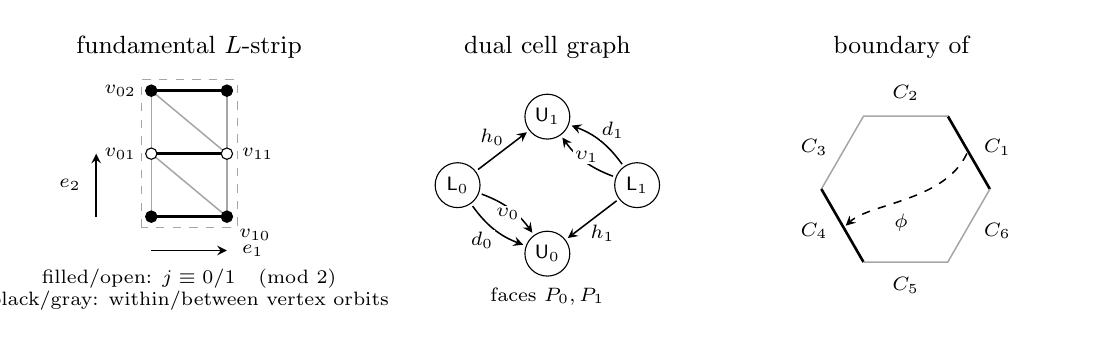
\begin{tikzpicture}[
  every node/.style={font=\scriptsize},
  panel title/.style={font=\small},
  orbit zero vertex/.style={circle,draw,fill=black,inner sep=1.45pt},
  orbit one vertex/.style={circle,draw,fill=white,inner sep=1.45pt},
  within orbit edge/.style={black,line width=0.95pt},
  between orbit edge/.style={gray!70,line width=0.55pt},
  dual vertex/.style={circle,draw,fill=white,minimum size=5.7mm,inner sep=0pt},
  dual edge/.style={->,line width=0.55pt,shorten <=1pt,shorten >=1pt},
  graph label/.style={fill=white,inner sep=0.7pt},
  identification/.style={dashed,->,line width=0.55pt,shorten <=1.5pt,shorten >=1.5pt},
  >=stealth]
\path[use as bounding box] (-2.05,-1.52) rectangle (11.15,2.05);

% The fundamental strip and its two residue classes modulo two.
\begin{scope}
  \node[panel title] at (0,1.80) {fundamental $L$-strip};
  \draw[dashed,gray!70] (-0.61,-0.49) rectangle (0.61,1.39);
  \draw[between orbit edge] (-0.48,-0.35)--(-0.48,1.25) (0.48,-0.35)--(0.48,1.25);
  \draw[between orbit edge] (0.48,-0.35)--(-0.48,0.45) (0.48,0.45)--(-0.48,1.25);
  \draw[within orbit edge] (-0.48,-0.35)--(0.48,-0.35) (-0.48,0.45)--(0.48,0.45) (-0.48,1.25)--(0.48,1.25);
  \node[orbit zero vertex] at (-0.48,-0.35) {};
  \node[orbit zero vertex] at (0.48,-0.35) {};
  \node[orbit one vertex] at (-0.48,0.45) {};
  \node[orbit one vertex] at (0.48,0.45) {};
  \node[orbit zero vertex] at (-0.48,1.25) {};
  \node[orbit zero vertex] at (0.48,1.25) {};
  \node[below right=1pt] at (0.48,-0.35) {$v_{10}$};
  \node[left=2pt] at (-0.48,0.45) {$v_{01}$};
  \node[right=2pt] at (0.48,0.45) {$v_{11}$};
  \node[left=2pt] at (-0.48,1.25) {$v_{02}$};
  \draw[->,line width=0.55pt] (-0.48,-0.78)--(0.48,-0.78);
  \node[right=2pt] at (0.48,-0.78) {$e_1$};
  \draw[->,line width=0.55pt] (-1.18,-0.35)--(-1.18,0.45) node[midway,left=2pt] {$e_2$};
  \node[align=center] at (0,-1.28) {filled/open: $j\equiv0/1\pmod2$\\black/gray: within/between vertex orbits};
\end{scope}

% The quotient dual graph and its translation labels.
\begin{scope}[xshift=4.55cm]
  \node[panel title] at (0,1.80) {dual cell graph};
  \node[dual vertex] (L0) at (-1.14,0.05) {$\mathsf L_0$};
  \node[dual vertex] (U0) at (0,-0.82) {$\mathsf U_0$};
  \node[dual vertex] (L1) at (1.14,0.05) {$\mathsf L_1$};
  \node[dual vertex] (U1) at (0,0.92) {$\mathsf U_1$};
  \draw[dual edge] (L0) to[bend right=17] (U0);
  \draw[dual edge] (L0) to[bend left=17] (U0);
  \draw[dual edge] (L0) -- (U1);
  \draw[dual edge] (L1) to[bend left=17] (U1);
  \draw[dual edge] (L1) to[bend right=17] (U1);
  \draw[dual edge] (L1) -- (U0);
  \node[graph label] at (-0.83,-0.65) {$d_0$};
  \node[graph label] at (-0.50,-0.31) {$\upsilon_0$};
  \node[graph label] at (-0.70,0.66) {$h_0$};
  \node[graph label] at (0.83,0.75) {$d_1$};
  \node[graph label] at (0.50,0.41) {$\upsilon_1$};
  \node[graph label] at (0.70,-0.56) {$h_1$};
  \node at (0,-1.36) {faces $P_0,P_1$};
\end{scope}

% The boundary hexagon on the normalization of a component.
\begin{scope}[xshift=9.10cm]
  \node[panel title] at (0,1.80) {boundary of $\dP$};
  \coordinate (c0) at (1.07,0); \coordinate (c1) at (0.535,0.927);
  \coordinate (c2) at (-0.535,0.927); \coordinate (c3) at (-1.07,0);
  \coordinate (c4) at (-0.535,-0.927);
  \coordinate (c5) at (0.535,-0.927);
  \draw[within orbit edge] (c0)--(c1);
  \draw[between orbit edge] (c1)--(c2)--(c3);
  \draw[within orbit edge] (c3)--(c4);
  \draw[between orbit edge] (c4)--(c5)--(c0);
  \node[right=2pt] at (0.80,0.53) {$C_1$};
  \node[above=2pt] at (0,0.927) {$C_2$};
  \node[left=2pt] at (-0.80,0.53) {$C_3$};
  \node[left=2pt] at (-0.80,-0.53) {$C_4$};
  \node[below=2pt] at (0,-0.927) {$C_5$};
  \node[right=2pt] at (0.80,-0.53) {$C_6$};
  \draw[identification] (0.80,0.50) .. controls (0.50,-0.15) and (-0.45,-0.18) .. node[pos=0.54,below=1pt] {$\phi$} (-0.80,-0.50);
\end{scope}
\end{tikzpicture}
\caption{The cusp for the index-two lattice.  In the left panel, the middle
horizontal edge is the diagonal $[v_{01},v_{11}]$ selected by
$\mathcal T$, and the dashed
rectangle is a fundamental region for
$L=\mathbb Ze_1\oplus\mathbb Z(2e_2)$.  The middle panel is the quotient
dual graph.  In the indicated edge order
$(d_0,\upsilon_0,h_0,d_1,\upsilon_1,h_1)$, its translation labels are
$(0,-e_1,-2e_2,0,-e_1,0)$.  In the right panel, the two heavy curves
$C_1,C_4$ are identified by $\phi$ to form a double curve of the
component, while $C_2+C_3+C_5+C_6$ maps to its intersection with the other
component.}
\label{fig:cusp-combinatorics}
\end{figure}
\FloatBarrier

The local fan construction is the same as in the saturated case.  What must
be checked here is that a proper finite-index sublattice still acts freely
and properly discontinuously and that the quotient remains proper over the
disc.  The following lemma records this form of the toric compactification;
compare \citep[Theorem~4.5]{Alpoge2026}.

\begin{lemma}[Toric compactification at the cusp]\label{lem:an-finite-index-cusp}
Let $\mathcal T$ be the periodic triangulation just defined, and let
$\Sigma$ be the fan in
$K_{\mathbb R}\oplus\mathbb R$ consisting of the cones over its faces
at height one.  Let $B_0:\ZZ^2\to K$ be injective with finite-index
image, and let $C(t)$ be a holomorphic $2$-by-$2$ matrix near zero.
The height character $t:=\chi^{(0,1)}$ extends to a holomorphic map
$t:X_\Sigma\to\CC$.  On the dense torus, write $x$ for the coordinate
in the two-dimensional torus with cocharacter lattice $K$, and define
\begin{equation}\label{eq:an-toric-action}
 \Psi_\lambda(x,t)
 =\bigl(e^{2\pi iC(t)\lambda}t^{B_0\lambda}x,t\bigr),
 \qquad \lambda\in\ZZ^2,
\end{equation}
where exponentials and powers are taken coordinatewise in the chosen basis
of $K$.  The maps extend to biholomorphisms.  For sufficiently
small $\epsilon>0$, their action on
$X_{\Sigma,\epsilon}:=\{|t|<\epsilon\}$ is free and properly
discontinuous, and
$X_{\Sigma,\epsilon}/\ZZ^2\to\{|t|<\epsilon\}$ is a proper map from a
smooth complex threefold.  Its central fibre is a reduced divisor with
normal crossings.
\end{lemma}

\begin{proof}
The integral shear $(y,r)\mapsto(y+rB_0\lambda,r)$
preserves $\Sigma$: at height one it translates $\mathcal T$ by the
lattice element $B_0\lambda$.  The induced toric map, composed with the
torus translation in \eqref{eq:an-toric-action}, gives the desired
extension.  The shear is the identity on the fibre cocharacter lattice and
fixes $t$, so it commutes with the torus factor.  These extensions form a
$\ZZ^2$-action because $\lambda\mapsto C(t)\lambda$ is additive.

For $t\ne0$, put $y=\log|x|/\log|t|$, coordinatewise; this is the
normalized logarithmic coordinate.  Then
\begin{equation}\label{eq:an-log-coordinate-translation}
 y\longmapsto y+B_t\lambda,
 \qquad
 B_t=B_0-\frac{2\pi\Im C(t)}{\log|t|}.
\end{equation}
Since $B_0$ is invertible over $\mathbb R$, shrinking $\epsilon$
gives a constant $a>0$ such that
\begin{equation}\label{eq:an-singular-value-bound}
 \|B_t\lambda\|\geq a\|\lambda\|
 \qquad(0<|t|<\epsilon,\ \lambda\in\ZZ^2).
\end{equation}
Hence the action is free on the dense torus.  A boundary
orbit is indexed by a bounded face $P$ of $\mathcal T$, and
$\Psi_\lambda$ carries it to the orbit indexed by
$P+B_0\lambda$.  No nonzero translation stabilizes a bounded face, so
the action is free on the boundary as well.

For proper discontinuity, let
$\sigma=\{v_0,v_1,v_2\}$.  Unimodularity identifies its chart with
$\CC^3$, with coordinates $z_0,z_1,z_2$ satisfying
\begin{equation}\label{eq:an-local-t-equation}
 t=z_0z_1z_2.
\end{equation}
If $\theta_i^\sigma$ are the barycentric coordinates of $\sigma$, then
on the dense torus
\begin{equation}\label{eq:an-barycentric-chart}
 \log|z_i|=\log|t|\,\theta_i^\sigma(y).
\end{equation}
Write
$U_\sigma(S)=\{|z_i|<S\text{ for }i=0,1,2\}
\cap X_{\Sigma,\epsilon}$.
Every point of $X_{\Sigma,\epsilon}$ lies in the closed unit polydisc of
some chart.  For a torus point, choose a triangle containing $y$.  For a
point on the orbit of a face $P$, choose a triangle containing $P$ whose
quotient cone contains the negative logarithmic coordinate normal to that
orbit.  Equation \eqref{eq:an-barycentric-chart} gives the assertion in
both cases.

If
$\Psi_\lambda U_\sigma(2)\cap U_{\sigma'}(2)\ne\varnothing$, density
gives such an intersection with $t\ne0$.  Formula
\eqref{eq:an-barycentric-chart} places the two normalized logarithmic
coordinates in
fixed bounded enlargements of $\sigma$ and $\sigma'$; their difference
is $B_t\lambda$.  The lower bound
\eqref{eq:an-singular-value-bound} therefore bounds $\lambda$ for each
fixed pair $(\sigma,\sigma')$.  The sets $U_\sigma(2)$ form an open
cover.  Given two compact sets, choose
finite subcovers of each by these sets and apply the bound to the finitely
many resulting pairs of triangles.  Only finitely many group elements can
move one compact set to meet the other, which proves proper discontinuity.

For properness over the disc, first suppose $t\ne0$ and choose
$\lambda$ so that
$B_t^{-1}y+\lambda\in[-1/2,1/2]^2$.
Uniform upper bounds on $B_t$ then put the translated logarithmic coordinate
in a fixed ball.  At $t=0$, use the finite set
$K/B_0\ZZ^2$: translating a face makes one of its vertices belong to a
fixed set of coset representatives.  Local finiteness of $\mathcal T$
then leaves only finitely many adjacent triangles.  Consequently, for each
$0<\epsilon_1<\epsilon$, every orbit over
$|t|\leq\epsilon_1$ meets
\begin{equation*}
 \mathcal K_0=
 \bigcup_{\sigma\in\mathcal F}
 \{|z_0|,|z_1|,|z_2|\leq1,\ |t|\leq\epsilon_1\},
\end{equation*}
where $\mathcal F$ is a finite family of triangles.  This is compact in
$X_{\Sigma,\epsilon}$, and its image is the full inverse image of the
closed subdisc.  The quotient map to the disc is therefore proper.

Each of the two triangle types has determinant $1$ or $-1$, so
$\Sigma$ is unimodular and $X_\Sigma$ is smooth.  The free quotient is
smooth.  The fan is countable, so $X_\Sigma$ has a countable toric atlas;
the quotient map is open, and the quotient is therefore second countable.
Since every ray generator has height one,
\eqref{eq:an-local-t-equation} gives a reduced normal crossings central
fibre.
\end{proof}

In this application the lemma's local height coordinate $t$ is
$t_c$.  Apply Lemma~\ref{lem:an-finite-index-cusp} to
\eqref{eq:an-cusp-period-splitting}--\eqref{eq:an-cusp-C}.  Denote the
quotient by $N_0\to\mathbb D_{t_c}$.
By \eqref{eq:an-index-two-image}, the vertices have two orbits, so the
central fibre has two irreducible components.  The identity point
$(1,1)$ extends across the toric model.  Indeed, in the chart for the
triangle $\{0,e_1,e_2\}$, the coordinates are
$z_0=t_c/(x_1x_2)$, $z_1=x_1$, and $z_2=x_2$.
The curve $(x_1,x_2,t_c)=(1,1,t_c)$ tends to $(0,1,1)$.  Its image
is a holomorphic section over the cusp disc, which we use as the origin in
the gluing.

For a height-one vertex $v$, let $E_v$
be the corresponding toric divisor and let $D_{[v]}$ be its image in the
quotient.  The star of $v$ has six primitive rays and is the complete fan
of $\dP$, so $E_v\cong\dP$ is compact and normal.  The map
$E_v\to D_{[v]}$ is surjective, is proper with finite fibres by proper
discontinuity, and is one-to-one over the dense orbit because no nonzero
translation fixes $v$.  It is therefore finite and birational, hence is
the normalization of $D_{[v]}$.  The two edges in the
$\pm\widehat w$-directions join vertices whose second coordinates are
congruent modulo two.  Their opposite boundary curves are identified to give
a double curve of $D_{[v]}$.  The other four edge directions join vertices
whose second coordinates are not congruent modulo two and map to the
intersection with the other component.  In a
triangle chart $t_c=z_0z_1z_2$, two vertices agree modulo two in their
second coordinates and the third does not, so the corresponding divisors
have local equations
$z_0z_1=0$ and $z_2=0$.  Thus the nonnormal double curve of
$D_{[v]}$ is ordinary and unramified, including at the triple points.

\subsection{The two multiple fibres}

The change of lattice must also be compatible with the finite monodromies.
Over the orbifold coordinate $s_j$, the linear action fixes the origin of
the torus and would produce a singular quotient.  The translation by
$v_j/m_j$ is chosen to produce a free affine action.  We must verify that this
action has order $m_j$, that its quotient has central divisor $m_jS_j$
with $S_j$ smooth, and that away from the central fibre it agrees with the
family $J$.  These are the properties needed to retain the multiplicities
three and four after passing from $\Lambda$ to $\Lambda^+$.

We apply to $\Lambda^+$ the logarithmic-transform construction described in
\citep[Definition~5.3 and Theorem~5.4]{Alpoge2026}, and verify freeness and
the identifications over the punctured discs.

On a small disc about $z_j$, the torus family defined by
\eqref{eq:an-period-matrix} extends across $s_j=0$.  Define a holomorphic
action on it by
\begin{equation}\label{eq:an-holomorphic-affine-action}
 \widetilde g_j(z,\zeta)
 =\left(g_jz,
 R_j(z)\zeta+\Pi^+(g_jz)\frac{v_j}{m_j}\right).
\end{equation}
Equation \eqref{eq:an-period-equivariance} makes this action well defined
modulo the periods.  In flat coordinates it is
$\widetilde g_j(z,x)=(g_jz,A_jx+v_j/m_j)$.
By \eqref{eq:an-finite-orders}, its $m_j$-th power is translation by
$v_j\in\Lambda^+$, hence the identity on the torus.

By \eqref{eq:an-finite-orders}, $\gamma\circ A_j^k=\gamma$.  A fixed point
of the $k$-th power can occur
only over $s_j=0$, and it would imply
$(A_j^k-I)x+kv_j/m_j\in\Lambda^+$.
Applying $\gamma$ would give
$k\gamma(v_j)/m_j\in\ZZ$.  For $j=1$, the two values are
$1/3,2/3$; for $j=2$, the three values are
$-1/4,-1/2,-3/4$.  None is integral.  Thus both cyclic actions, including
all their nonidentity elements, are free.

Let $N_j$ be the quotient by this cyclic action.  It is smooth and proper
over the disc with coordinate $t_j=s_j^{m_j}$.
Indeed, before quotienting the family is, in real flat coordinates, a
bundle of compact real four-tori; over every compact subdisc its total
space is compact, and a finite quotient preserves properness.  Since the
quotient is \'etale and
$\operatorname{div}(s_j^{m_j})=m_j\{s_j=0\}$, its central divisor is
$m_jS_j$, with $S_j$ smooth and reduced.

To glue this model to $J$, we identify their restrictions over the
punctured disc.  On a simply connected sector of the punctured $s_j$-disc,
choose a branch of the logarithm and put
$\ell(z)=\log s_j(z)/(2\pi i)$.
On the $g_j$-translates of the chosen sector, choose compatible branches
satisfying $\ell(g_jz)=\ell(z)-1/m_j$.  Translation in the torus by
$\ell(z)\Pi^+(z)v_j$
conjugates \eqref{eq:an-holomorphic-affine-action} to the linear action.
Indeed, $A_jv_j=v_j$ and
\eqref{eq:an-period-equivariance} give
$\Pi^+(g_jz)v_j/m_j+\ell(g_jz)\Pi^+(g_jz)v_j
=R_j(z)\ell(z)\Pi^+(z)v_j$.
Changing the logarithm changes the translation
$\ell(z)\Pi^+(z)v_j$ by the period $\Pi^+(z)v_j$.  It therefore descends to
the torus and identifies $N_j\setminus S_j$ with $J$ over the punctured
disc.  The zero section of $J$ extends across the cusp as the holomorphic
section constructed above; we use this zero section in all three
identifications over the punctured discs.

\subsection{Identification over the punctured cusp and global gluing}

The torus family $J$ is written in additive period coordinates, whereas
the toric model $N_0$ is written in multiplicative coordinates with
cocharacter lattice $K$.  To glue them, we must show that exponentiation
first quotients by $K$ and the cusp monodromy and that the residual deck
action is exactly the action used in the toric construction.  This identifies
the two models over a punctured cusp disc.

On the chosen component $\widetilde U_0$, consider
\begin{equation}\label{eq:an-cusp-exponential-map}
 (s,\zeta)\longmapsto
 \bigl(t_c=e^{2\pi is},\ x=e^{2\pi i\zeta}\bigr),
\end{equation}
where the second exponential is coordinatewise.  It quotients the last two
period columns of \eqref{eq:an-period-matrix}.  It also quotients the base
deck transformation because $s(g_0z)=s(z)-1$ and
$R_{g_0}=I$.  Its kernel is the subgroup $H$ generated
by $g_0$ and the period lattice
$K=\mathbb Z\widehat w\oplus\mathbb Zd$.  Equations
\eqref{eq:an-cusp-monodromy-interface} give
$A_0|_K=I$ and $(A_0-I)\Lambda^+\subset K$, so $H$ is normal in the
deck group over the cusp,
$G_c=\Lambda^+\rtimes_{A_0}\langle g_0\rangle$.  The quotient
$G_c/H$ is $\Lambda^+/K\cong\mathbb Z^2$.  By
\eqref{eq:an-cusp-period-splitting}, it acts by
$x\longmapsto e^{2\pi iC^+(t_c)\lambda}
t_c^{B_0^+\lambda}x$, where $\lambda\in\ZZ^2$,
which is the toric action \eqref{eq:an-toric-action}.  Hence
\eqref{eq:an-cusp-exponential-map} induces a biholomorphism between the
restriction of $J$ to a punctured cusp disc and the punctured restriction
of $N_0$.

We use the gluing procedure of \citep[Construction~6.1]{Alpoge2026},
replacing the cusp model associated with $\Lambda$ by the one constructed
above for $\Lambda^+$.

\begin{proof}[Proof of Proposition~\ref{prop:analytic-model}]
Choose pairwise disjoint coordinate discs $U_j$ around the three marked
points.  Glue $J$, $N_0$, $N_1$, and $N_2$ by the three
biholomorphisms over $U_j\setminus\{p_j\}$, and call the result
$Y$.  The transition maps are biholomorphic, and distinct local models do
not overlap, so they give a smooth complex-manifold atlas.

The glued space is Hausdorff.  Two points with different images in $B$
are separated by inverse images
of disjoint base neighbourhoods.  Two points over the same base point lie
in a single Hausdorff model: over each $U_j$ the glued space is exactly
$N_j$, with no second copy of the central fibre, while away from the
marked points it is $J$.  It is second countable because only finitely many
second-countable spaces were glued along open subsets.

The map $f:Y\to B$ is locally one of the proper maps constructed above.
Properness is local on the target for maps between locally compact
Hausdorff spaces, so $f$ is proper.  Since $B$ is compact, $Y$ is
compact.  The space $J$ is connected, and every local model meets it over a
punctured disc, so $Y$ is connected.  The descriptions of the three
special fibres proved above give all the remaining assertions of the
proposition.
\end{proof}
